
\documentclass[11pt,a4paper]{article}

\usepackage[T1]{fontenc}
\usepackage[utf8]{inputenc}
\usepackage{amsmath,amssymb,amsthm}
\usepackage{booktabs}
\usepackage{array}
\usepackage{graphicx}
\usepackage{tikz}
\usepackage{url}
\usepackage{geometry}

\geometry{margin=1in}
\usetikzlibrary{arrows.meta,positioning,calc,shapes.geometric}

\setlength{\parskip}{0.45em}
\setlength{\parindent}{1.5em}
\renewcommand{\arraystretch}{1.15}

\newtheorem{definition}{Definition}[section]
\newtheorem{proposition}[definition]{Proposition}
\newtheorem{theorem}[definition]{Theorem}
\newtheorem{corollary}[definition]{Corollary}
\newtheorem{lemma}[definition]{Lemma}
\newtheorem{assumption}[definition]{Assumption}
\newtheorem{remark}[definition]{Remark}
\newtheorem{conjecture}[definition]{Conjecture}

\title{\textbf{The Theory of Gainful Distillation}\\
\large The Science of Learning and Intelligence}
\author{Soumadeep Ghosh}
\date{14 November 2026}

\begin{document}
\maketitle

\begin{abstract}
Conventional knowledge distillation is commonly formulated as the transfer of predictive information from a teacher model to a student model. This treatise develops a broader framework: \emph{Gainful Distillation}, in which a teacher coordinates a network of five heterogeneous students, learns the students' learning dynamics, allocates instructional and computational resources, receives verified discoveries from its students, and updates its own knowledge and teaching policies. The system is designed not merely to reproduce a teacher's outputs, but to increase the verified capability of the collective learning system while preserving useful diversity, independent inquiry, safety, and economic efficiency.

The proposed network has six vertices: one teacher and five students. The students form a complete graph \(K_5\), augmented by an additional circumferential overlay. The overlay is represented as an additional structural channel on each perimeter pair, so that the five perimeter pairs have multiplicity two while the five diagonals have multiplicity one. The topology is fixed in the baseline model, whereas directed transmission intensities adapt over time. Teacher-to-student and student-to-teacher influence are distinct, and peer influence is recipient-specific.

The treatise integrates adaptive learning-rate estimation, the Ghoshian Dual Parallel State--Attention Architecture, Breadth--Depth learning dynamics, specialist task routing, constrained resource allocation, uncertainty-aware transmission, independent validation, and an informational-governance process. It derives sufficient conditions for contraction in a simplified error-propagation model, formulates a local spectral stability criterion for the complete feedback system, and proposes a welfare objective that accounts for capability gain, innovation, compute, coordination, and risk. It also develops a reproducible econometric programme with matched-compute baselines, ablations, clustered uncertainty estimates, causal interventions, and explicit falsification criteria.

The disciplinary discussions extend to control theory, physics, chemistry, biology, educational psychology, psychiatry, linguistics, philosophy, comparative religion, law, public policy, international relations, diplomacy, cybersecurity, and the economics of security. These connections are distinguished as mathematical imports, empirical hypotheses, institutional analogies, or ethical constraints; metaphor is not treated as scientific evidence. The central conjecture is that a well-governed, stability-constrained learning network can achieve positive net capability gain over its original teacher when its verified learning benefits exceed its computational, coordination, and error costs. This is a research programme, not a claim of completed empirical proof.
\end{abstract}

\noindent\textbf{Keywords:} knowledge distillation; meta-learning; learning to teach; multi-agent learning; adaptive control; graph theory; state-space models; Transformer; resource allocation; innovation; epistemic diversity; AI governance.

\tableofcontents
\newpage

\section{Introduction}

\subsection{From compression to capability creation}

Knowledge distillation has an established meaning in machine learning: a student is trained to reproduce useful aspects of a teacher's predictive behaviour, often through softened output distributions \cite{hinton2015,bucilua2006}. Ensemble compression and specialist models show that useful predictive structure can be transferred without deploying every original model at inference time \cite{hinton2015}. Yet the teacher--student metaphor need not end with compression. Born-Again Neural Networks demonstrate that a student trained with a teacher-derived objective can, under particular experimental conditions, outperform the teacher \cite{furlanello2018}. That result motivates a larger question: can the whole teacher--student system be organised so that improvement is an explicit objective rather than an incidental outcome?

This treatise proposes an affirmative, but testable, architecture. The teacher is an executive coordinator and an active learner. Each student is a general learner with a developing comparative advantage. The teacher estimates how each student learns, not merely how well it performs. Students exchange information, work independently, collaborate on complex tasks, and submit discoveries for external validation. The teacher can learn from these discoveries and from successful student learning strategies.

The system is called the \emph{Gainful Distillation System} (GDS). Its objective is not maximal agreement. It is verified, sustainable, system-level learning gain.

\subsection{The Xerox problem and the coin-flipper problem}

A system that rewards only agreement with its teacher risks producing highly competent replicas. A system that rewards novelty without verification risks producing confident but unreliable claims. The design problem is therefore two-sided: avoid mere reproduction and avoid unconstrained speculation.

Ghosh's fuzzy-logic treatment of the ``coin-flipper'' and the ``Xerox machine'' formalises two limiting failures: performance indistinguishable from chance and high-scoring reproduction without origination \cite{ghosh2026gpa}. Its stylised optimum is a result of that paper's specified membership functions and product t-norm. It is not a universal target score for AI models, nor does its numerical GPA optimum transfer to machine learning. Its conceptual lesson is that competence and independent contribution should be assessed jointly rather than inferred from a single score.

Accordingly, GDS distinguishes:
\begin{enumerate}
\item predictive competence on established tasks;
\item generalisation to unseen tasks and distributions;
\item calibrated uncertainty and error detection;
\item independently verified discoveries;
\item transfer of knowledge across domains;
\item efficiency and resilience under a fixed resource budget.
\end{enumerate}

\subsection{Research status and epistemic discipline}

The architecture contains established components, proposed integrations, and conjectures. Standard distillation, graph methods, recursive estimation, convex optimisation, and local stability analysis have established mathematical foundations. The particular six-agent architecture, its transmission rules, the proposed Student Learning Dynamics Estimator, and the Gainful Distillation Conjecture are proposals requiring empirical testing. No theorem in this treatise establishes that a five-student network will outperform a single model in every domain.

\section{Conceptual foundations and related work}

\subsection{Knowledge distillation and specialist models}

In classical distillation, teacher and student predictive distributions are compared, often using a temperature-scaled Kullback--Leibler divergence \cite{hinton2015}. Earlier work on model compression established that a compact model can approximate an ensemble's function \cite{bucilua2006}. Specialist models and ensemble methods motivate heterogeneous expertise rather than identical replicas. GDS retains the teacher--student loss but embeds it in a larger objective that includes independent task performance, peer exchange, verified novelty, and cost.

\subsection{Meta-learning and learning to teach}

Meta-learning studies how learning procedures themselves can be adapted from experience. Model-Agnostic Meta-Learning provides a general method for learning initial parameters that adapt rapidly to new tasks \cite{finn2017}. The GDS extension is institutional as well as parametric: the teacher learns which instructional interventions work for which student, domain, and training stage. The teacher's policy is therefore a learned policy over teaching actions.

\subsection{Ghoshian Dual Parallel State--Attention Architecture}

The Ghoshian Dual Parallel State--Attention Architecture (G-DPSA) combines Transformer-based attention, State Space Model memory, adaptive fusion, executive control, reinforcement learning, hierarchical memory, and mixture-of-experts routing \cite{ghosh2026gdpsa}. In the present treatise, each student may instantiate a G-DPSA-like internal architecture. This is an optional model family, not a requirement that all five students share identical internals.

A representative dual pathway is
\begin{align}
h_{i,t}^{T} &= T_{\theta_i^T}(x_t),\\
h_{i,t}^{S} &= S_{\theta_i^S}(x_t),\\
h_{i,t} &= g_{i,t}h_{i,t}^{T}+(1-g_{i,t})h_{i,t}^{S},\\
g_{i,t} &= R_{\phi_i}(B_{i,t},D_{i,t}),
\end{align}
where \(B_{i,t}\) and \(D_{i,t}\) denote Breadth and Depth state variables. The fusion gate \(g_{i,t}\) is learned or controlled from the student's current learning state.

\subsection{Breadth and Depth as candidate state variables}

Ghosh's empirical validation programme proposes that Breadth and Depth may be measurable state variables with predictive and potentially causal relationships to future learning gains \cite{ghosh2026empirical}. It recommends predictive tests, information-theoretic analysis, orthogonalisation against conventional training variables, interventions, phase diagrams, and an efficient frontier. GDS adopts this as an empirical hypothesis, not as an established law of learning.

For student \(i\), a generic future gain at horizon \(k\) is
\begin{equation}
Y_{i,t}^{(k)}=L_{i,t}-L_{i,t+k},
\end{equation}
where \(L_{i,t}\) is a consistently measured held-out loss. A positive value indicates loss reduction. Breadth and Depth are useful only if they add predictive or causal information beyond baseline covariates such as loss, gradient norm, learning rate, compute, and data exposure.

\section{The six-agent graph}

\subsection{Vertices and structural topology}

Let
\begin{equation}
V=\{T,S_1,S_2,S_3,S_4,S_5\},
\end{equation}
where \(T\) is the teacher and \(S_i\) are five students. The students form a complete graph \(K_5\). An additional circumferential overlay connects the five students in cyclic order. This overlay is an extra channel, not merely a restatement of the perimeter edges already present in \(K_5\).

In the vertex order \(T,S_1,S_2,S_3,S_4,S_5\), the structural adjacency matrix is
\begin{equation}
A=
\begin{pmatrix}
0&1&1&1&1&1\\
1&0&2&1&1&2\\
1&2&0&2&1&1\\
1&1&2&0&2&1\\
1&1&1&2&0&2\\
1&2&1&1&2&0
\end{pmatrix}.
\end{equation}
The five student perimeter pairs have multiplicity two: one ordinary \(K_5\) edge and one circumferential overlay channel. The five diagonals have multiplicity one. Each teacher--student pair has one structural channel. The total multiplicity is twenty. The teacher's weighted degree is five; each student's weighted degree is seven.

\subsection{Graph illustration}

\begin{figure}[ht]
\centering
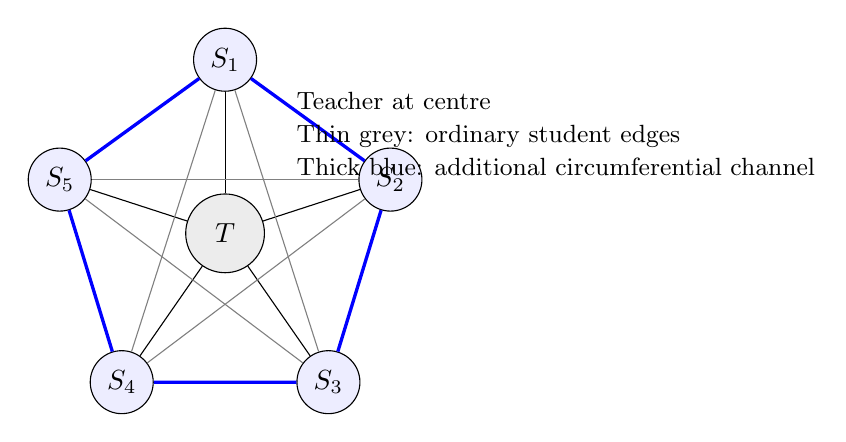
\begin{tikzpicture}[scale=1.05, every node/.style={circle,draw,minimum size=8mm,inner sep=1pt},
  teacher/.style={circle,draw,fill=gray!15,minimum size=10mm},
  student/.style={circle,draw,fill=blue!7,minimum size=8mm},
  every edge/.style={draw,thin}]
\node[teacher] (T) at (0,0) {\(T\)};
\node[student] (S1) at (0,2.1) {\(S_1\)};
\node[student] (S2) at (2.0,0.65) {\(S_2\)};
\node[student] (S3) at (1.25,-1.8) {\(S_3\)};
\node[student] (S4) at (-1.25,-1.8) {\(S_4\)};
\node[student] (S5) at (-2.0,0.65) {\(S_5\)};
\foreach \s in {S1,S2,S3,S4,S5} \draw (T)--(\s);
\foreach \a/\b in {S1/S2,S1/S3,S1/S4,S1/S5,S2/S3,S2/S4,S2/S5,S3/S4,S3/S5,S4/S5}
  \draw[gray] (\a)--(\b);
\foreach \a/\b in {S1/S2,S2/S3,S3/S4,S4/S5,S5/S1}
  \draw[very thick,blue] (\a)--(\b);
\node[draw=none,rectangle,align=left] at (4.0,1.2) {\small Teacher at centre\\\small Thin grey: ordinary student edges\\\small Thick blue: additional circumferential channel};
\end{tikzpicture}
\caption{Six-agent topology. Thick perimeter strokes overlay, rather than replace, the ordinary \(K_5\) edges.}
\label{fig:network}
\end{figure}

\subsection{Static topology and dynamic transmission}

The topology is fixed in the baseline model, but the transmission intensities are directed and time-varying. Let \(W_t\) be a \(6\times6\) matrix of directed transmission strengths. Its entries distinguish teacher-to-student, student-to-teacher, and peer-to-peer influence:
\begin{align}
(W_t)_{T,S_i}&=\tau_{i,t},\\
(W_t)_{S_i,T}&=\nu_{i,t},\\
(W_t)_{S_i,S_j}&=A_{ij}\kappa_{ij,t},\qquad i\ne j.
\end{align}
In general,
\begin{equation}
\tau_{i,t}\ne\nu_{i,t},
\qquad
\kappa_{ij,t}\ne\kappa_{ji,t}.
\end{equation}
The factor \(A_{ij}\) preserves the structural multiplicity. If the two perimeter channels later receive different adaptive multipliers, the single effective term \(2\kappa_{ij,t}\) can be decomposed into two channel-specific terms.

\section{Student learning dynamics}

\subsection{A student is a learning system, not a static score}

Represent student \(i\) by
\begin{equation}
S_i=
(\theta_i^T,\theta_i^S,\phi_i,M_i,E_i,\mathcal P_i),
\end{equation}
where \(\theta_i^T\) and \(\theta_i^S\) are Transformer and SSM parameters, \(\phi_i\) is an executive controller, \(M_i\) is memory, \(E_i\) is a set of specialist modules, and \(\mathcal P_i\) is a record of validated learning strategies.

The teacher should estimate a vector of student learning characteristics rather than a single scalar learning rate:
\begin{equation}
\boldsymbol{\ell}_{i,d,m,t}
=
\left(
\eta_{i,d,m,t},
\rho_{i,d,t},
\chi_{i,d,t},
\mu_{i,d,t},
\zeta_{i,d,m,t},
B_{i,t},
D_{i,t}
\right)^\top.
\end{equation}
Here \(d\) denotes a task domain and \(m\) an instructional method. The components may represent effective learning rate, retention, transfer, memory utilisation, responsiveness to instructional support, Breadth, and Depth. These are operational constructs to be measured, not claims about subjective experience.

\subsection{Learning rate versus estimated learning rate}

The actual effective learning rate is not directly observed by the teacher. The teacher maintains a posterior or filtered estimate:
\begin{equation}
\widehat{\boldsymbol{\ell}}_{i,d,m,t}
=
\mathbb E[
\boldsymbol{\ell}_{i,d,m,t}\mid\mathcal H_t
],
\end{equation}
where \(\mathcal H_t\) is the history of interventions, task conditions, observations, and outcomes. An uncertainty covariance matrix \(P_{i,d,m,t}\) accompanies the estimate.

The teacher should not treat a point estimate as certainty. Instructional decisions should account for posterior uncertainty and should sometimes select informative interventions that improve the estimate.

\subsection{A local response model}

Let \(u_{i,t}\) denote an instructional intervention, such as a worked derivation, conceptual explanation, retrieval exercise, counterexample, independent research task, or peer collaboration. For a fixed domain and local operating region, use
\begin{equation}
\Delta Q_{i,t}
=
\eta_{i,t}u_{i,t}+\varepsilon_{i,t},
\end{equation}
where \(\Delta Q_{i,t}\) is a measured learning gain and \(\varepsilon_{i,t}\) is observation noise. This is a local approximation, not a global law of neural learning.

A recursive least-squares update is
\begin{align}
K_{i,t}
&=
\frac{P_{i,t-1}u_{i,t}}
{\sigma_i^2+u_{i,t}^2P_{i,t-1}},\\
\widehat{\eta}_{i,t}
&=
\widehat{\eta}_{i,t-1}
+
K_{i,t}
\left(
\Delta Q_{i,t}
-u_{i,t}\widehat{\eta}_{i,t-1}
\right),\\
P_{i,t}
&=
(1-K_{i,t}u_{i,t})P_{i,t-1}.
\end{align}
This scalar update assumes a linear response, known noise variance, and sufficiently informative interventions. A multivariate estimator is required when interventions interact or learning rates vary substantially by task.

\subsection{Teacher as a learner of learning strategies}

The teacher learns not only the response function of each student but also which instructional methods are effective. Let \(\mathcal P_{i,t}\) be the set of candidate strategies associated with student \(i\). A strategy is promoted to the validated strategy repository only after replicated evidence:
\begin{equation}
\mathcal P_t^{\mathrm{verified}}
=
\bigcup_{i=1}^{5}
\left\{
p\in\mathcal P_{i,t}:
\operatorname{Replicated}(p)=1
\right\}.
\end{equation}
A strategy that works for one student is not automatically universal. The teacher estimates heterogeneity and transfer conditions before generalising it.

\section{The Student Learning Dynamics Estimator}

\subsection{Purpose}

The Student Learning Dynamics Estimator (SLDE) is the subsystem by which the teacher learns how each student learns. It performs seven functions:
\begin{enumerate}
\item estimates domain- and method-specific learning responses;
\item estimates retention and transfer;
\item tracks Breadth and Depth trajectories;
\item estimates uncertainty and data sufficiency;
\item measures the marginal effectiveness of instructional interventions;
\item updates teacher-to-student support intensity;
\item detects strategies that may transfer to other students.
\end{enumerate}

\subsection{Instructional policy}

The teacher selects a support action by solving
\begin{equation}
u_{i,t}^{*}
=
\arg\max_{u\in\mathcal U_i}
\left\{
\mathbb E[\Delta Q_{i,t}\mid u,\widehat{\boldsymbol{\ell}}_{i,t}]
-\lambda_u C(u)
-\lambda_r\mathcal R(u)
\right\},
\end{equation}
where \(C(u)\) is the computational cost and \(\mathcal R(u)\) is the estimated risk of the intervention. The policy should also account for the value of information when an intervention is informative about an uncertain learning parameter.

A more complete Bayesian decision criterion is
\begin{equation}
u_{i,t}^{*}
=
\arg\max_{u\in\mathcal U_i}
\left\{
\mathbb E[\Delta Q_{i,t}\mid u]
+\lambda_{\mathrm{info}}\operatorname{VOI}(u)
-\lambda_u C(u)
-\lambda_r\mathcal R(u)
\right\}.
\end{equation}
Here \(\operatorname{VOI}(u)\) is the expected value of information obtained by observing the student's response to \(u\). It is not always optimal to choose the intervention with the highest immediate gain; a carefully chosen diagnostic task may improve later instructional decisions.

\subsection{Learning-rate matching}

The following table gives illustrative, testable instructional hypotheses. It does not classify students permanently.

\begin{table}[ht]
\centering
\small
\begin{tabular}{p{0.24\linewidth}p{0.30\linewidth}p{0.35\linewidth}}
\toprule
Observed pattern & Candidate interpretation & Candidate support policy\\
\midrule
Fast short-run gain, weak delayed retention & Acquisition exceeds consolidation & Retrieval practice, spaced review, memory checks\\
Slow gain, strong retention & Gradual but durable acquisition & Structured sequencing and adequate training horizon\\
High Breadth, low Depth & Broad exploration without consolidation & Focused derivations and proof tasks\\
Low Breadth, high Depth & Narrow but developed competence & Carefully selected cross-domain transfer tasks\\
Strong independent discoveries & High autonomous contribution & Greater research autonomy and independent validation\\
Large peer-learning effect & Collaboration is informative & Specialist pairing and structured peer exchange\\
\bottomrule
\end{tabular}
\caption{Illustrative learning-response patterns and adaptive support.}
\end{table}

\section{Adaptive transmission}

\subsection{Source value and recipient-specific relevance}

A student's general capability does not determine its value as a source for every recipient. Let the value of source \(i\) to recipient \(j\) be
\begin{equation}
z_{ij,t}
=
a_1Q_{i,t}
+a_2V_{i,t}
+a_3M_{ij,t}
+a_4U_{i,t}
-a_5R_{ij,t},
\end{equation}
where \(Q_{i,t}\) is independently measured capability, \(V_{i,t}\) is verification reliability, \(M_{ij,t}\) is recipient-specific marginal information value, \(U_{i,t}\) is an exploration bonus, and \(R_{ij,t}\) is estimated transmission risk.

For a student recipient \(j\), define peer probabilities
\begin{equation}
p_{ij,t}
=
(1-\epsilon_p)
\frac{A_{ij}\exp(z_{ij,t}/T_p)}
{\sum_{k\in\mathcal N_j^S}A_{kj}\exp(z_{kj,t}/T_p)}
+
\frac{\epsilon_p}{|\mathcal N_j^S|},
\end{equation}
where \(\mathcal N_j^S\) is the set of peer students connected to \(j\), \(T_p>0\) is a temperature, and \(0<\epsilon_p<1\) is an exploration floor. The probabilities sum to one over eligible peers. The exploration floor prevents a low-ranked student from becoming permanently disconnected.

\subsection{Teacher-to-student transmission}

Teacher-to-student intensity should depend on the verified knowledge gap, the student's estimated learning response, the task domain, and the marginal value of instruction. One bounded specification is
\begin{equation}
\tau_{j,t}
=
\tau_{\min}
+
(\tau_{\max}-\tau_{\min})
\sigma\left(
b_1G_{j,t}
+b_2C_{j,t}
+b_3\operatorname{VOI}_{j,t}
-b_4M_{j,t}
\right),
\end{equation}
where \(G_{j,t}\) is a knowledge gap, \(C_{j,t}\) is estimated instructional receptivity, \(M_{j,t}\) is demonstrated mastery, and \(\sigma(x)=(1+\exp(-x))^{-1}\). The terms must be domain-specific and calibrated. Mastery should reduce redundant instruction, not reduce access to challenging work.

\subsection{Student-to-teacher transmission}

The teacher's attention to student submissions should reflect capability, verification, novelty, knowledge-gap relevance, uncertainty, and risk:
\begin{equation}
e_{i,t}
=
c_1Q_{i,t}
+c_2V_{i,t}
+c_3O_{i,t}
+c_4G_{i,t}
-c_5R_{i,t}.
\end{equation}
A bounded attention allocation is
\begin{equation}
\nu_{i,t}
=
(1-\epsilon_T)
\frac{\exp(e_{i,t}/T_T)}
{\sum_{j=1}^{5}\exp(e_{j,t}/T_T)}
+
\frac{\epsilon_T}{5}.
\end{equation}
Thus \(\sum_i\nu_{i,t}=1\) and every student retains a positive minimum attention share. This is an allocation of investigative attention, not automatic acceptance of a student's claims.

\subsection{Transmission, investigation, and integration}

Every student submission passes through three logically distinct stages:
\begin{enumerate}
\item \textbf{Transmission:} the finding is submitted with provenance, assumptions, uncertainty, and reproducible artefacts.
\item \textbf{Investigation:} independent checks evaluate correctness, novelty, scope, robustness, and possible correlated error.
\item \textbf{Integration:} only findings that satisfy the relevant verification standard enter the trusted knowledge base.
\end{enumerate}
The system retains rejected and unresolved findings in an auditable record. A finding is not true merely because it is novel, and it is not false merely because it contradicts the teacher.

\section{Task specialisation and coalition formation}

\subsection{Comparative advantage}

Each student remains a general learner while developing a comparative advantage. Let \(q\) index a task and let
\begin{equation}
s_i(q,t)
=
f_i(q,\widehat{\boldsymbol{\ell}}_{i,t},B_{i,t},D_{i,t},\mathcal H_{i,t})
\end{equation}
be the estimated suitability of student \(i\). A softmax router assigns
\begin{equation}
\pi_i(q,t)
=
\frac{\exp(s_i(q,t)/T_r)}
{\sum_{j=1}^{5}\exp(s_j(q,t)/T_r)}.
\end{equation}
For tasks that benefit from collaboration, choose a coalition \(\mathcal C(q,t)\subseteq\{S_1,\ldots,S_5\}\). Coalition value must include complementarity, coordination costs, and correlated failure risk.

\subsection{Coalition value}

Let \(Q(\mathcal C,q)\) be independently measured coalition performance and \(C(\mathcal C,q)\) its cost. A coalition is preferred when
\begin{equation}
\mathcal V(\mathcal C,q)
=
Q(\mathcal C,q)
-\lambda_C C(\mathcal C,q)
-\lambda_R R(\mathcal C,q)
\end{equation}
exceeds the value of the best feasible individual assignment. This makes collaboration an empirical decision rather than a presumption that more agents are always better.

\section{Resource allocation and financial planning}

\subsection{Budget constraints}

Let \(r_{i,t}\) be compute or research resources allocated to student \(i\), and \(R_t\) the total available budget:
\begin{align}
r_{i,t}&\geq \underline r_i\geq0,\\
\sum_{i=1}^{5}r_{i,t}&\leq R_t.
\end{align}
The lower bound is optional and should be imposed only when maintaining a specialist capability or exploration path has strategic value.

\subsection{Mean--variance allocation}

Let \(\mu_{i,t}\) be expected marginal verified capability gain per unit of resource and \(\Sigma_t\) the covariance matrix of marginal gains. A proposed resource-allocation programme is
\begin{equation}
\max_{\mathbf r_t}
\left\{
\boldsymbol{\mu}_t^\top\mathbf r_t
-\frac{\lambda_r}{2}\mathbf r_t^\top\Sigma_t\mathbf r_t
-\frac{\eta_r}{2}\|\mathbf r_t\|_2^2
\right\}
\end{equation}
subject to the budget and capacity constraints. The covariance term penalises correlated returns; the quadratic regulariser discourages extreme concentration. This is a GDS extension of constrained resource-allocation reasoning, not the identical optimisation problem in Ghosh's paper on stochastic resource allocation \cite{ghosh2026resource}.

\subsection{Convexity and solution conditions}

\begin{proposition}
If \(\Sigma_t\) is positive semidefinite, \(\lambda_r\geq0\), and \(\eta_r>0\), then the objective in the resource-allocation programme is strictly concave in \(\mathbf r_t\). If the feasible set is nonempty and compact, a unique maximiser exists.
\end{proposition}
\begin{proof}
The Hessian of the objective is
\begin{equation}
H_t=-\lambda_r\Sigma_t-\eta_r I.
\end{equation}
For any nonzero vector \(x\),
\begin{equation}
x^\top H_tx
=
-\lambda_r x^\top\Sigma_tx-\eta_r\|x\|_2^2<0,
\end{equation}
because \(\Sigma_t\) is positive semidefinite and \(\eta_r>0\). Hence the objective is strictly concave. A continuous strictly concave function on a nonempty compact convex feasible set has a unique maximiser.
\end{proof}

\subsection{Financial planning interpretation}

The GDS budget should be managed as a portfolio of learning investments. The relevant unit is not raw tokens, training steps, or GPU-hours in isolation, but verified marginal capability gain per unit of total cost. The budget should distinguish:
\begin{itemize}
\item fixed costs: model hosting, orchestration, secure storage, evaluation infrastructure;
\item variable costs: training, inference, tool calls, data acquisition, validation;
\item risk reserves: incident response, rollback, independent audits, reproducibility;
\item research reserves: exploratory tasks and underrepresented domains;
\item maintenance: model refresh, security patches, dataset governance, and monitoring.
\end{itemize}
A financial plan should report expected, adverse, and stress scenarios. Forecasts must not treat uncertain innovation as guaranteed revenue or capability.

\section{Error propagation and stability}

\subsection{Five-student peer error model}

Let \(e_{i,t}\) be the deviation of student \(i\)'s estimate from an independently validated target, and let \(\mathbf e_t\) collect the five errors. Consider the simplified model
\begin{equation}
\mathbf e_{t+1}
=
(qI+\beta P_t)\mathbf e_t+\boldsymbol{\xi}_t,
\end{equation}
where \(0\leq q<1\) is local error persistence, \(\beta\geq0\) is peer-error transmission strength, \(P_t\) is a nonnegative row-stochastic matrix, and \(\boldsymbol{\xi}_t\) is a disturbance.

\begin{theorem}[Sufficient contraction condition]
If \(P_t\) is row-stochastic and \(q+\beta<1\), then the homogeneous peer-error system is a contraction in the infinity norm. If disturbances satisfy \(\|\boldsymbol{\xi}_t\|_\infty\leq\bar\xi\), then
\begin{equation}
\limsup_{t\rightarrow\infty}\|\mathbf e_t\|_\infty
\leq
\frac{\bar\xi}{1-q-\beta}.
\end{equation}
\end{theorem}
\begin{proof}
Because \(P_t\) is nonnegative and row-stochastic, its induced infinity norm is one. By the triangle inequality and submultiplicativity,
\begin{align}
\|\mathbf e_{t+1}\|_\infty
&\leq
\|qI+\beta P_t\|_\infty\|\mathbf e_t\|_\infty
+\|\boldsymbol{\xi}_t\|_\infty\\
&\leq
(q+\beta)\|\mathbf e_t\|_\infty+\bar\xi.
\end{align}
Iterating this scalar inequality gives
\begin{equation}
\|\mathbf e_t\|_\infty
\leq
(q+\beta)^t\|\mathbf e_0\|_\infty
+
\bar\xi\sum_{k=0}^{t-1}(q+\beta)^k.
\end{equation}
Since \(q+\beta<1\), the first term converges to zero and the geometric sum converges to \(1/(1-q-\beta)\). This proves the bound.
\end{proof}

\begin{remark}
This is a sufficient condition for a simplified linear model. It is not a universal stability theorem for neural-network training. Nonlinear learning, changing data distributions, delayed feedback, adaptive optimisers, and nonstationary transmission matrices require local Jacobian, Lyapunov, or input-to-state stability analysis.
\end{remark}

\subsection{Six-agent local stability}

Let \(\mathbf z_t\) collect teacher and student errors. A local linearisation around an operating point yields
\begin{equation}
\mathbf z_{t+1}=H_t\mathbf z_t+\boldsymbol{\zeta}_t.
\end{equation}
For a time-invariant local approximation, a standard asymptotic stability condition is
\begin{equation}
\rho(H)<1,
\end{equation}
where \(\rho(H)\) is the spectral radius. For time-varying \(H_t\), uniform bounds on products of transition matrices or an appropriate common Lyapunov function are needed. The complete system must be analysed because teacher feedback can amplify or damp student errors.

\subsection{Diversity and anti-collapse constraints}

A stable network can still collapse into intellectual homogeneity. Let \(h_i\) denote a representation or capability profile and \(\bar h\) its mean. Define
\begin{equation}
\mathcal D_t
=
\frac{1}{5}\sum_{i=1}^{5}\|h_i-\bar h\|^2.
\end{equation}
A minimum diversity constraint may be used:
\begin{equation}
\mathcal D_t\geq\underline{\mathcal D}.
\end{equation}
The objective is not arbitrary disagreement. Diversity should be task-relevant and should improve collective performance or robustness. The system should preserve independent learning:
\begin{equation}
L_{i,t}
=
\lambda_{T,i,t}L_{T\rightarrow i}
+\lambda_{P,i,t}L_{\mathrm{peer},i}
+\lambda_{I,i,t}L_{\mathrm{ind},i},
\qquad
\lambda_{I,i,t}\geq\underline\lambda_I>0.
\end{equation}
This prevents teacher and peer imitation from consuming the entire learning process.

\section{Innovation, latent capability, and verification}

\subsection{Capability is multidimensional}

A student's capability profile should include accuracy, generalisation, calibration, robustness, transfer, reasoning validity, specialist competence, efficiency, and independently verified discovery. A single benchmark score cannot identify all these dimensions.

\subsection{Public metrics and latent capability}

A public metric may fail to reveal capabilities encoded in internal representations. Ghosh's work on asymmetric metrics motivates comparing observable benchmark performance with information recoverable from learned representations. Such a gap can motivate further tests, but it is not itself proof of intelligence, originality, or general capability. A representation probe may exploit leakage, spurious structure, or distribution-specific information. Every latent-capability claim requires out-of-distribution validation and an independent test.

A generic metric gap is
\begin{equation}
\Delta_i^{\mathrm{metric}}
=
L_i^{\mathrm{public}}-L_i^{\mathrm{representation}},
\end{equation}
where the two losses are measured under carefully controlled data splits and comparable evaluation protocols.

\subsection{Asymmetric innovation}

Ghosh's Asymmetric Innovation Score proposes an asymmetric treatment of upside, downside dispersion, and benchmark mimicry \cite{ghosh2026innovation}. With semi-deviations \(\sigma^+\) and \(\sigma^-\), and positive benchmark correlation \(\rho^+\), the score is
\begin{equation}
I(f;w)=\alpha\sigma^+-\beta(\sigma^-)^2-\gamma\rho^+.
\end{equation}
This score can be adapted as one feature in the GDS innovation assessment. It must not be interpreted as a complete measure of scientific novelty. Correlation with a teacher can indicate copying, shared evidence, or simply common correctness. Conversely, disagreement can indicate innovation or error. Novelty therefore requires independent verification, not correlation alone.

\subsection{Verified discovery score}

Let \(O_{i,t}\) denote a discovery score that is zero until the relevant verification threshold is passed. One possible decomposition is
\begin{equation}
O_{i,t}
=
N_{i,t}C_{i,t}^{*}R_{i,t}^{*}G_{i,t}^{*},
\end{equation}
where \(N\) measures novelty, \(C^*\) correctness, \(R^*\) reproducibility, and \(G^*\) generalisation. The multiplicative form makes a zero in a critical dimension suppress the final score. In applications, a vector of verification results may be preferable to a single scalar.

\section{Informational ethics and epistemic governance}

\subsection{Information gaps as investigation programmes}

Ghosh's Asymmetric Informational Ethics (AIE) treats ethical activity as a set of programmes initiated by informational asymmetries, advanced through investigation, and terminated only when relevant asymmetries and outstanding decisions are exhausted \cite{ghosh2026aie}. GDS adopts this process-oriented insight for model governance.

Let \(\mathcal A_t\) be the set of unresolved informational asymmetries and \(\mathcal D_t\) the set of outstanding decisions. A governance programme is not complete merely because a model emits an answer. It is complete when the relevant evidence has been investigated, the decision has been made or explicitly deferred, and the residual uncertainty is documented.

\subsection{Epistemic state machine}

\begin{figure}[ht]
\centering
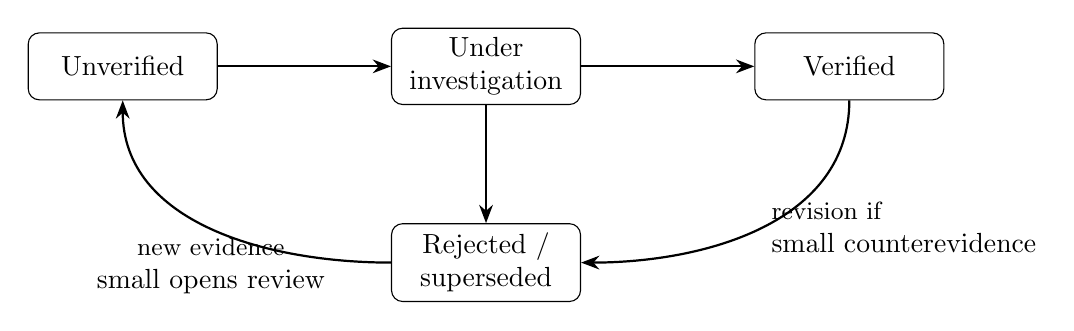
\begin{tikzpicture}[node distance=2.2cm,>=Stealth,
  box/.style={draw,rounded corners,align=center,minimum width=2.4cm,minimum height=0.85cm},
  arr/.style={->,thick}]
\node[box] (u) {Unverified};
\node[box,right=of u] (i) {Under\\investigation};
\node[box,right=of i] (v) {Verified};
\node[box,below=1.5cm of i] (r) {Rejected /\\superseded};
\draw[arr] (u)--(i);
\draw[arr] (i)--(v);
\draw[arr] (i)--(r);
\draw[arr] (r.west) to[out=180,in=270] node[below,align=center] {\small new evidence\\small opens review} (u.south);
\draw[arr] (v.south) to[out=270,in=0] node[right,align=left] {\small revision if\\small counterevidence} (r.east);
\end{tikzpicture}
\caption{A minimal evidence-status process. Rejection is retained in the audit history; verification is revisable when new evidence warrants it.}
\label{fig:epistemic}
\end{figure}

\subsection{Non-domination by the teacher}

The teacher is an executive coordinator, not an infallible epistemic sovereign. It may request evidence, challenge an inference, allocate additional testing, and update its own knowledge. It may not reject a result solely because the result contradicts its existing parameters or outputs. Independent validation is necessary precisely because teacher and students may share training data, architecture, blind spots, or incentives.

\subsection{Ethical principles}

The system should implement:
\begin{enumerate}
\item proportionality between the task's legitimate purpose and the resources or risks involved;
\item data minimisation and purpose limitation;
\item traceability of training data, model versions, tool use, and material claims;
\item contestability and a documented appeal path;
\item non-discrimination testing across relevant groups and languages;
\item protection of confidential information and intellectual property;
\item human accountability for consequential decisions;
\item incident reporting, rollback, and remediation.
\end{enumerate}
These principles are consistent with the broad human-rights and accountability orientation of the UNESCO Recommendation on the Ethics of Artificial Intelligence \cite{unesco2021} and risk-management approaches such as the NIST AI Risk Management Framework \cite{nist2023}. The precise legal duties depend on jurisdiction, sector, and deployment context.

\section{Economics, welfare, and strategic resource use}

\subsection{System welfare}

Let \(Q_{\mathcal G,t}\) be collective capability measured on a held-out evaluation suite and \(Q_{T,0}\) the original teacher's baseline capability. Define
\begin{equation}
\Delta Q_{\mathcal G,t}=Q_{\mathcal G,t}-Q_{T,0}.
\end{equation}
Let \(O_{\mathcal G,t}\) be verified innovation, \(E_{\mathcal G,t}\) efficiency, \(R_{\mathcal G,t}\) risk, \(C_{\mathcal G,t}\) compute cost, and \(L_{\mathcal G,t}\) coordination and validation overhead. A welfare objective is
\begin{align}
\mathcal W_t={}&
\alpha_Q\Delta Q_{\mathcal G,t}
+\alpha_O O_{\mathcal G,t}
+\alpha_E E_{\mathcal G,t}\\
&-\alpha_R R_{\mathcal G,t}
-\alpha_C C_{\mathcal G,t}
-\alpha_L L_{\mathcal G,t}.
\end{align}
The weights require transparent calibration. Since a scalar welfare index embeds value judgments, the study should also report a Pareto frontier and disaggregated outcomes.

\subsection{Gainful Distillation Conjecture}

\begin{conjecture}[Gainful Distillation]
Under suitable conditions on task heterogeneity, estimator quality, resource sufficiency, validation reliability, and feedback stability, an adaptive teacher--student network with independent learning and specialist allocation can achieve greater expected net welfare than the original teacher operating alone under an equivalent resource budget.
\end{conjecture}

A compact statement of the conjecture is
\begin{equation}
\mathbb E[\mathcal W_{\mathrm{GDS}}]
>
\mathbb E[\mathcal W_{\mathrm{teacher}}],
\end{equation}
where both systems are evaluated under comparable resource constraints and the same external test distribution. This is a falsifiable research claim, not a theorem established by the present derivations.

\subsection{Public economics and distributional incidence}

A system may raise aggregate capability while concentrating access, compute, income, or decision power. Welfare evaluation should therefore report distributional incidence: who receives benefits, who bears costs, which languages and domains are underserved, and whether smaller institutions can access the resulting capabilities. Efficiency does not by itself establish fairness. Where feasible, report subgroup outcomes, access costs, and the distribution of model errors.

\subsection{Warfare economics and strategic restraint}

The same resource-allocation mathematics can describe defensive resilience, logistics, risk analysis, and crisis communication. This treatise does not derive operational targeting, weapons employment, or offensive military procedures. For high-consequence security applications, the objective should prioritise lawful defensive resilience, escalation prevention, civilian protection, auditability, and human command responsibility. A model that improves tactical efficiency while increasing catastrophic risk is not welfare-improving under a defensible social objective.

\section{Disciplinary connections}

\subsection{Mathematics, logic, and proof theory}

The core mathematical objects are weighted directed graphs, stochastic matrices, constrained optimisation problems, Bayesian estimators, and dynamical systems. Formal logic supplies a discipline for separating premises, derivations, and conclusions. A model-generated proof should be checked by a proof assistant, symbolic computation, or independent derivation when the result is consequential. Syntactic validity is not semantic truth.

\subsection{Physics and control theory}

The stability analysis is mathematically related to feedback control. Transmission gains act like coupling coefficients; disturbances act like external inputs; the spectral radius or a Lyapunov function can describe local stability. This is a structural analogy with precise mathematical content. It does not imply that model representations are physical fields or that computational learning obeys thermodynamic laws without an explicit physical model.

A compute budget has a physical cost: energy consumption, heat dissipation, cooling, hardware wear, and infrastructure. The engineering objective should therefore include energy and thermal constraints:
\begin{equation}
E_{\mathrm{total}}
=
\sum_{i=1}^{5}E_i+E_T+E_{\mathrm{network}}+E_{\mathrm{validation}}.
\end{equation}
The system's energy efficiency can be reported as verified capability gain per joule, alongside latency and monetary cost.

\subsection{Chemistry and material constraints}

Chemistry enters through the physical infrastructure rather than through an unsupported claim that neural learning is a chemical reaction. Semiconductor fabrication, battery chemistry, cooling fluids, corrosion, and material supply chains constrain the hardware ecosystem. Life-cycle assessment should account for embodied materials, electricity mix, water use, cooling, and electronic waste. These variables belong in the cost and sustainability ledger.

\subsection{Biology and evolutionary adaptation}

The system's exploration, specialisation, and retention have limited analogies with variation, selection, and adaptation. The analogy is useful only at the level of abstract processes. Artificial students are engineered computational systems, not organisms; evolutionary language must not obscure the absence of biological metabolism, reproduction, or intrinsic welfare. Population diversity can nevertheless motivate the preservation of alternative hypotheses and specialist competencies.

\subsection{Psychology, education, and psychiatry}

Educational psychology motivates measurement of acquisition, retention, transfer, feedback, cognitive load, and practice effects. The SLDE should use behavioural and computational observables rather than anthropomorphic assumptions. A student's measured learning curve is not a diagnosis of a human learner. Psychiatry concerns human clinical conditions and cannot be inferred from model loss, representations, or response patterns. If human participants are involved in evaluation, appropriate research ethics, informed consent, privacy protection, and qualified clinical oversight are required.

\subsection{Linguistics and multilingual capability}

Language competence should be evaluated across syntax, semantics, pragmatics, discourse, translation, morphology, and culturally situated usage. A shared benchmark can conceal large differences between languages and dialects. Specialist routing may therefore be language- and domain-aware, while independent evaluation should include native-speaker assessment and cross-lingual transfer. The teacher must not treat high-resource-language performance as a universal proxy for linguistic intelligence.

\subsection{Philosophy and epistemology}

The architecture raises questions about knowledge, justification, testimony, disagreement, and intellectual authority. Teacher outputs are testimony, not axioms. Student disagreement is a reason to investigate, not a proof of correctness. Knowledge integration should distinguish truth, justified belief, confidence, reproducibility, and decision usefulness. The system should preserve uncertainty where evidence is insufficient.

\subsection{Religion and comparative ethics}

Religious traditions contain diverse accounts of knowledge, duty, compassion, restraint, humility, stewardship, and the moral limits of power. These traditions are internally plural and cannot be reduced to one algorithmic reward function. GDS can support respectful comparative study and multilingual access to religious texts, but must not claim theological authority, collapse traditions into a single doctrine, or infer a person's religious identity from their data. The normative core of deployment remains subject to human rights, lawful governance, and pluralistic deliberation.

\subsection{Political science, geopolitics, and diplomacy}

The six-agent system is a small institutional network with differentiated roles, unequal information, and mechanisms for agenda-setting and dispute resolution. Its governance resembles a deliberative institution more than a sovereign hierarchy. International deployment raises questions of jurisdiction, data sovereignty, export controls, language access, research collaboration, and strategic dependence. Cross-border cooperation should favour interoperable standards, independent evaluation, transparent incident reporting, and diplomatic channels for resolving disputes.

\subsection{Law and institutional accountability}

The GDS architecture does not determine legal personhood or transfer legal responsibility to models. Accountability remains with the relevant human and organisational actors under applicable law. Deployment analysis should consider data protection, confidentiality, intellectual property, consumer protection, product safety, discrimination, employment, research integrity, and sector-specific regulation. This treatise is not jurisdiction-specific legal advice. Legal review must be conducted for each deployment territory and use case.

\subsection{Cybersecurity}

The network creates a larger attack surface: model endpoints, shared memory, training data, tool interfaces, evaluation pipelines, update channels, and inter-agent messages. Threats include data poisoning, prompt injection, model extraction, credential compromise, supply-chain compromise, denial of service, and malicious or accidental cross-agent propagation.

Minimum controls include:
\begin{itemize}
\item least-privilege identity and access management;
\item signed model, dataset, and configuration artefacts;
\item isolated execution for untrusted tools and code;
\item provenance and integrity checks for peer messages;
\item secrets management and encryption in transit and at rest;
\item rate limits, anomaly detection, and audit logging;
\item independent red-team exercises and incident response;
\item rollback and recovery procedures for model and data updates.
\end{itemize}
Peer-to-peer trust should be earned through authenticated provenance and validation, not inferred from network membership.

\section{Econometrics and empirical identification}

\subsection{Experimental models}

The principal comparison should include:
\begin{table}[ht]
\centering
\small
\begin{tabular}{p{0.10\linewidth}p{0.48\linewidth}p{0.30\linewidth}}
\toprule
Model & Architecture & Identified contribution\\
\midrule
M0 & Original teacher alone & Baseline capability and cost\\
M1 & Five independent students & Parallel learning without distillation\\
M2 & Teacher and five students; no peer exchange & Teacher-to-student transfer\\
M3 & Teacher, \(K_5\), overlay, adaptive routing and resource allocation & Collaboration and allocation\\
M4 & Full GDS with SLDE, adaptive transmission, independent learning, verification and governance & Integrated architecture\\
\bottomrule
\end{tabular}
\caption{Matched-budget experimental baselines.}
\end{table}

All models should receive comparable total compute, data access, tuning opportunities, and evaluation exposure. If the systems differ in hardware or data quality, those differences must be recorded and controlled.

\subsection{Primary outcomes}

The primary outcomes are:
\begin{enumerate}
\item capability gain over the original teacher;
\item out-of-distribution and cross-domain transfer;
\item verified discoveries per unit of compute;
\item delayed retention;
\item calibration and selective prediction;
\item correlated error and propagation;
\item robustness under distribution shift and adversarial inputs;
\item teacher improvement attributable to student submissions;
\item cost, energy, latency, and coordination overhead;
\item subgroup and language-specific performance.
\end{enumerate}

\subsection{Panel specification}

Let \(i\) index students, \(d\) domains, \(t\) training windows, and \(k\) evaluation horizons. A panel model for future gain is
\begin{align}
Y_{i,d,t}^{(k)}
={}&\alpha_i+\delta_d+\tau_t
+\beta_1 B_{i,t}
+\beta_2 D_{i,t}
+\beta_3\widehat\eta_{i,d,t}\\
&+\beta_4 V_{i,t}
+\beta_5 O_{i,t}
+\boldsymbol{\gamma}^{\top}\mathbf X_{i,d,t}
+\varepsilon_{i,d,t},
\end{align}
where \(\alpha_i\), \(\delta_d\), and \(\tau_t\) are student, domain, and time effects, and \(\mathbf X\) includes baseline loss, gradient norm, compute, data exposure, task difficulty, and model size. Standard errors should account for clustering at the appropriate experimental unit. With only five students in one network, conventional large-sample cluster asymptotics are weak; replication across seeds, tasks, and independent networks is essential.

\subsection{Causal identification}

Predictive association does not establish that Breadth, Depth, or instructional method causes learning gain. Where feasible, randomise instructional interventions within student--domain blocks. Use pre-registered treatment definitions, common evaluation sets, and blinded scoring. A simple intervention estimand is
\begin{equation}
\operatorname{ATE}
=
\mathbb E[Y(1)-Y(0)],
\end{equation}
where \(Y(1)\) and \(Y(0)\) are potential outcomes under two specified instructional policies. Interference between students violates the simplest no-interference assumption; network experiments should therefore define exposure mappings or randomise at the network or cluster level.

\subsection{Ablation design}

Remove one component at a time while preserving compute budgets:
\begin{itemize}
\item adaptive teacher-to-student transmission;
\item adaptive student-to-teacher feedback;
\item peer transmission;
\item the additional circumferential overlay;
\item the SLDE;
\item specialist task routing;
\item independent learning;
\item Breadth--Depth control;
\item innovation scoring;
\item external validation and governance;
\item stability and concentration constraints.
\end{itemize}
Factorial designs may identify interactions, but the number of combinations should be balanced against compute and statistical power.

\subsection{Falsification criteria}

The architecture should be considered unsupported, or a component rejected, if:
\begin{enumerate}
\item full GDS fails to improve net welfare under matched resource budgets;
\item estimated learning profiles do not improve instructional decisions out of sample;
\item peer exchange increases correlated error more than it improves capability;
\item specialist routing fails to outperform non-specialist allocation on heterogeneous tasks;
\item innovation rewards increase unsupported novelty or benchmark exploitation;
\item the additional circumferential channels provide no reproducible marginal benefit;
\item validation overhead exceeds the value of the discoveries it certifies.
\end{enumerate}

\section{Algorithms and implementation}

\subsection{Recursive GDS procedure}

The following pseudocode describes a research implementation. It is deliberately abstract and does not prescribe a particular framework or hardware stack.

\begin{verbatim}
INITIALISE teacher T and students S[1..5]
INITIALISE structural adjacency A
INITIALISE directed transmission weights W
INITIALISE learning profiles Lhat[1..5]
INITIALISE uncertainty states P[1..5]
INITIALISE verified knowledge base K
INITIALISE discovery register R
INITIALISE resource budget B

FOR each training round t:

    OBSERVE student performance, loss, calibration,
            Breadth, Depth, retention, compute, and uncertainty

    UPDATE each student learning profile using SLDE
    ESTIMATE domain-specific instructional response
    ESTIMATE marginal verified gain and covariance

    ROUTE tasks to specialists or coalitions
    SOLVE constrained resource allocation problem

    FOR each student i:
        SELECT instructional intervention using Lhat[i]
        TRANSMIT teacher knowledge subject to risk limits
        TRANSMIT peer knowledge using recipient-specific weights
        TRAIN student with an independent-learning floor
        RECORD outcomes, costs, and provenance

    COLLECT student discoveries and learning strategies
    VALIDATE claims using independent tests
    UPDATE discovery register:
        unverified / investigating / verified / rejected

    INTEGRATE only verified findings into trusted knowledge
    UPDATE teacher using validated student contributions
    UPDATE directed transmission weights
    CHECK concentration, diversity, and stability constraints
    CHECK security, privacy, and governance controls

    EVALUATE collective capability on held-out tasks
    COMPUTE net welfare and uncertainty intervals
    STORE complete audit record

END FOR
\end{verbatim}

\subsection{Complexity and systems engineering}

For five students, the peer graph has ten unordered pairs and twenty directed peer channels. The graph-level orchestration overhead is small relative to foundation-model training, but model inference, validation, and data movement may dominate. Complexity should be measured empirically: graph size alone is not a proxy for system cost.

A practical implementation should separate:
\begin{enumerate}
\item orchestration and policy service;
\item model-serving layer;
\item student-specific memory and state;
\item secure message bus;
\item task router and coalition manager;
\item SLDE estimation service;
\item resource scheduler;
\item external validation service;
\item audit, monitoring, and incident-response systems.
\end{enumerate}

\section{Open mathematical problems}

The present framework leaves several substantial questions open.

\subsection{Joint equilibrium}

The teacher chooses instructional effort, students update parameters, and transmission weights respond to observed performance. A stationary equilibrium would require mutually consistent policies:
\begin{align}
\pi_T^*&\in\arg\max_{\pi_T}\mathbb E[\mathcal W\mid\pi_T,\pi_S,W],\\
\pi_S^*&\in\arg\max_{\pi_S}\mathbb E[\mathcal W\mid\pi_T,\pi_S,W],\\
W^*&=\Psi(\pi_T^*,\pi_S^*,\text{verified evidence}).
\end{align}
Existence and uniqueness require assumptions on compactness, continuity, convexity, and the update operator. They are not established here.

\subsection{Optimal exploration floor}

The exploration parameter \(\epsilon\) trades off exploitation of reliable sources against the possibility of discovering overlooked capability. Its optimal value may depend on task novelty, uncertainty, and the cost of experimentation. A contextual bandit or Bayesian experimental-design formulation is a natural candidate.

\subsection{Optimal number of students}

Five students are a design choice for the present architecture, not a universal optimum. Let \(n\) be the number of students. The optimal network size should solve
\begin{equation}
n^*
=
\arg\max_n
\left\{
\mathbb E[\Delta Q_n]
-\lambda_C C_n
-\lambda_L L_n
-\lambda_R R_n
\right\}.
\end{equation}
The marginal value of an additional student must exceed its compute, coordination, validation, and security costs.

\subsection{Dynamic topology}

The baseline model keeps topology fixed to isolate the value of adaptive transmission. A later extension may allow edges to be activated, attenuated, or retired. Any such change should preserve auditability and prevent strategic isolation of dissenting or low-ranked students.

\section{Limitations}

First, the learning profile is an operational statistical construct. It does not reveal a model's subjective experience, consciousness, or human-like psychological state. Second, a student's apparent learning rate may be confounded by task difficulty, data quality, compute, prompt format, evaluation noise, and parameter count. Third, teacher and student errors may be correlated through shared data and architecture. Fourth, innovation is difficult to measure: novelty, correctness, importance, and generality are distinct. Fifth, welfare weights encode normative choices and must be reported transparently. Sixth, legal obligations vary by jurisdiction. Seventh, analogies with biological, chemical, religious, or geopolitical systems are not evidence of literal equivalence.

\section{Conclusion}

The Theory of Gainful Distillation reframes distillation as a reciprocal and institutionally governed learning process. The teacher transmits knowledge, learns how each student learns, and adapts its instructional support. Students specialise without losing their general-learning capacity, collaborate without surrendering independent inquiry, and submit discoveries to independent validation. The teacher is capable of learning from them, including when their verified findings contradict its existing beliefs.

The five-student network is deliberately structured: a complete graph \(K_5\), an additional circumferential overlay, and a central teacher connected to every student. Its topology is distinguished from its directed, adaptive transmission strengths. The SLDE estimates domain- and method-specific learning responses. The resource allocator directs compute toward expected marginal verified gain while accounting for covariance, concentration, and minimum research capacity. Stability constraints limit error amplification; diversity and independent-learning constraints resist epistemic collapse; governance rules separate transmission from verification and integration.

The decisive criterion is not whether the students reproduce the teacher perfectly. It is whether the collective system becomes more capable, more reliable, more efficient, and more independently productive under a comparable resource budget. A perfect score is not necessarily evidence of a perfect learner. Nor is disagreement necessarily evidence of discovery. The system must reward neither imitation nor novelty in isolation, but verified learning and responsible contribution.

The central conjecture remains open to experiment. Its value lies partly in its falsifiability: if the network's gains do not exceed its costs and risks, the architecture must be revised or rejected. If they do, the teacher--student relationship becomes a reciprocal learning economy in which the teacher can improve its students, the students can improve their teacher, and the collective can develop capabilities that none possessed at the outset.

\section*{Acknowledgements and research status}

This treatise synthesises concepts from the author's cited manuscripts and the present collaborative design discussion. The proposed GDS, SLDE, transmission rules, stability constraints, and empirical hypotheses are new integrations in this document. They should be treated as a theoretical specification and research agenda until independently implemented and evaluated. No empirical superiority claim is made.

\section*{Glossary}
\begin{description}
\item[Adaptive transmission] A time-varying directed strength assigned to an information channel.
\item[Asymmetric innovation] An evaluation approach that distinguishes favourable outcomes, downside risk, and mimicry.
\item[Breadth] A candidate state variable intended to capture the breadth of a model's learning activity.\item[Coalition] A task-specific subset of students assigned to collaborate.
\item[Depth] A candidate state variable intended to capture the depth or consolidation of learning.
\item[Distillation] Transfer of predictive or representational information from one model to another.
\item[External Validation Layer] An independent mechanism for checking correctness, novelty, reproducibility, and generalisation.
\item[Gainful Distillation] Distillation designed to increase verified collective capability rather than merely reproduce teacher outputs.
\item[Knowledge gap] A measured difference between the knowledge or capability of a student and a relevant reference.
\item[Learning profile] A time-varying estimate of a student's domain- and method-specific learning dynamics.
\item[Learning-rate matching] Selection of instructional support using estimated student learning responses.
\item[Metric gap] A difference between performance measured by a public benchmark and information recoverable under a separate representation-based evaluation.
\item[Peer transmission] Directed transfer of information between students.
\item[SLDE] Student Learning Dynamics Estimator.
\item[Specialisation] Development of comparative advantage in a domain while retaining general learning capacity.
\item[Structural multiplicity] The number of distinct structural channels represented by an adjacency entry.
\item[Verified discovery] A novel contribution that has passed the applicable independent correctness and reproducibility checks.
\item[Welfare] A declared aggregate evaluation of capability, innovation, efficiency, cost, risk, and coordination.
\end{description}

\begin{thebibliography}{99}

\bibitem{bucilua2006}
C. Bucilu\u{a}, R. Caruana, and A. Niculescu-Mizil,
\newblock Model compression,
\newblock in \emph{Proceedings of the 12th ACM SIGKDD International Conference on Knowledge Discovery and Data Mining}, 2006, pp. 535--541.

\bibitem{finn2017}
C. Finn, P. Abbeel, and S. Levine,
\newblock Model-agnostic meta-learning for fast adaptation of deep networks,
\newblock in \emph{Proceedings of the 34th International Conference on Machine Learning}, PMLR 70, 2017, pp. 1126--1135.

\bibitem{furlanello2018}
T. Furlanello, Z. C. Lipton, M. Tschannen, L. Itti, and A. Anandkumar,
\newblock Born Again Neural Networks,
\newblock in \emph{Proceedings of the 35th International Conference on Machine Learning}, PMLR 80, 2018, pp. 1607--1616.

\bibitem{ghosh2026gdpsa}
S. Ghosh,
\newblock \emph{The Ghoshian Dual Parallel State--Attention Architecture: A Unified Cognitive, Economic, and Computational Framework for Adaptive Foundation Models},
\newblock author manuscript, 2026.

\bibitem{ghosh2026empirical}
S. Ghosh,
\newblock \emph{Empirical Validation of the Ghoshian Dual Parallel State--Attention Architecture},
\newblock author manuscript, 2026.

\bibitem{ghosh2026gpa}
S. Ghosh,
\newblock \emph{Between the Coin-Flipper and the Xerox Machine: The Optimal GPA via Fuzzy Logic on the Borel Algebra of [0,1]},
\newblock author manuscript, 2026.

\bibitem{ghosh2026resource}
S. Ghosh,
\newblock \emph{Optimal Resource Allocation in Stochastic Environments: A Multidisciplinary Analysis of Constrained Quadratic Optimization in Financial and Geopolitical Contexts},
\newblock author manuscript, 2026, with Qwen3.7.

\bibitem{ghosh2026innovation}
S. Ghosh,
\newblock \emph{An Asymmetric Innovation Score},
\newblock author manuscript, 2026.

\bibitem{ghosh2026metrics}
S. Ghosh,
\newblock \emph{Asymmetric Metrics},
\newblock author manuscript, 2026.

\bibitem{ghosh2026aie}
S. Ghosh,
\newblock \emph{The Complete Treatise on Asymmetric Informational Ethics},
\newblock author manuscript, 2026.

\bibitem{hinton2015}
G. Hinton, O. Vinyals, and J. Dean,
\newblock Distilling the Knowledge in a Neural Network,
\newblock \emph{NIPS Deep Learning and Representation Learning Workshop}, 2015.

\bibitem{kalman1960}
R. E. Kalman,
\newblock A new approach to linear filtering and prediction problems,
\newblock \emph{Journal of Basic Engineering}, vol. 82, no. 1, 1960, pp. 35--45.

\bibitem{boyd2004}
S. Boyd and L. Vandenberghe,
\newblock \emph{Convex Optimization},
\newblock Cambridge University Press, 2004.

\bibitem{pearl2009}
J. Pearl,
\newblock \emph{Causality: Models, Reasoning, and Inference}, 2nd ed.,
\newblock Cambridge University Press, 2009.

\bibitem{shannon1948}
C. E. Shannon,
\newblock A mathematical theory of communication,
\newblock \emph{Bell System Technical Journal}, vol. 27, 1948, pp. 379--423 and 623--656.

\bibitem{sutton2018}
R. S. Sutton and A. G. Barto,
\newblock \emph{Reinforcement Learning: An Introduction}, 2nd ed.,
\newblock MIT Press, 2018.

\bibitem{unesco2021}
UNESCO,
\newblock \emph{Recommendation on the Ethics of Artificial Intelligence},
\newblock adopted 23 November 2021.

\bibitem{nist2023}
National Institute of Standards and Technology,
\newblock \emph{Artificial Intelligence Risk Management Framework (AI RMF 1.0)},
\newblock NIST AI 100-1, 2023.

\bibitem{arrow1951}
K. J. Arrow,
\newblock \emph{Social Choice and Individual Values},
\newblock Wiley, 1951.

\bibitem{sen1999}
A. Sen,
\newblock \emph{Development as Freedom},
\newblock Oxford University Press, 1999.

\bibitem{ostrom1990}
E. Ostrom,
\newblock \emph{Governing the Commons: The Evolution of Institutions for Collective Action},
\newblock Cambridge University Press, 1990.

\end{thebibliography}

\end{document}